\chapter{Services Architecture} \label{ap1:annex-high-level-arch}

This annex contains the architecture diagram of the implemented solution, representing all of its components, as explained in Chapter~\ref{chap:solution}.

\begin{landscape}
    \begin{figure}
       \centering
        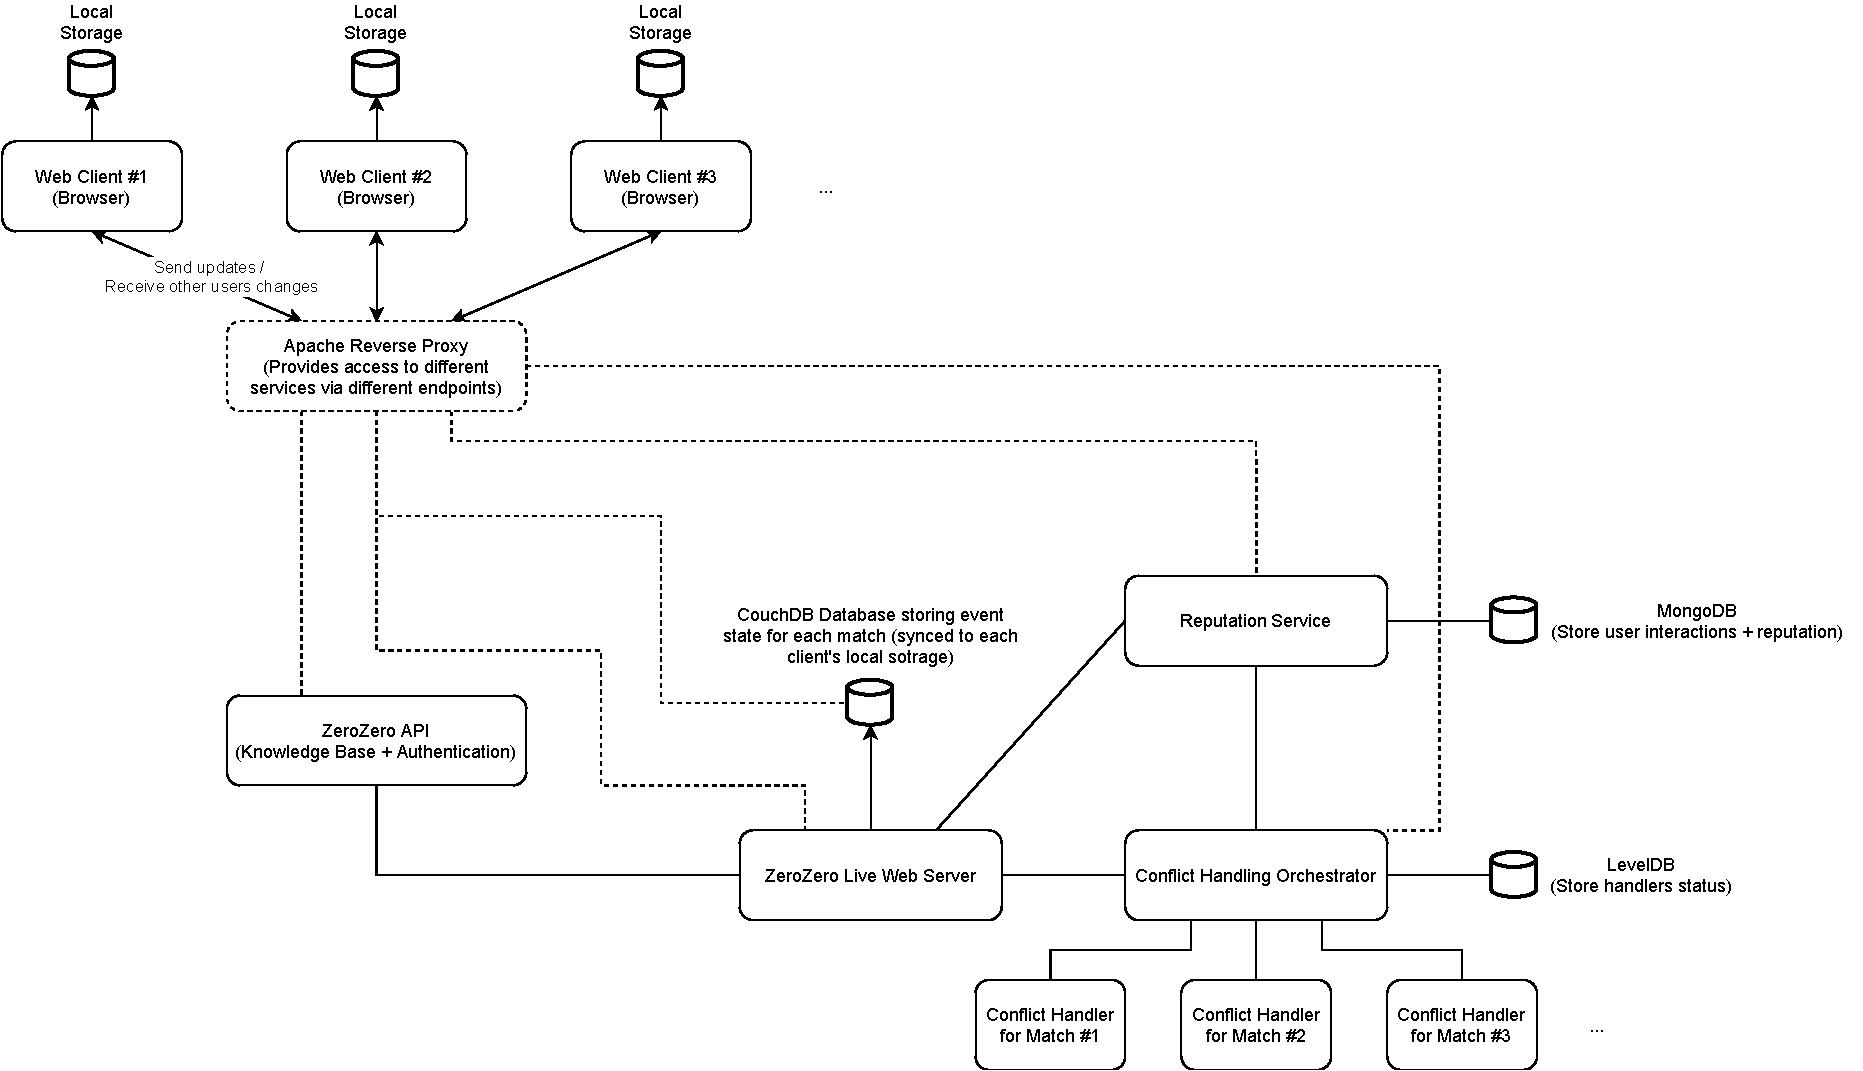
\includegraphics[height=0.9\textheight]{zerozerolive-arch.pdf}
        \caption{Services Architecture of the Application}
        \label{fig:annex-high-level-arch}
    \end{figure}
    \end{landscape}

\chapter{ZeroZero API events list} \label{annex:api-events}

\begin{longtable}{| p{.20\textwidth} | p{.60\textwidth} | p{.20\textwidth} |} 
    \caption{ZeroZero API events list (some fields were omitted for better reading purposes)} \\
    \hline
    \textbf{Event Id} & \textbf{Event Name} & \textbf{Category} \\ \hline
    \endfirsthead       
    \hline    
    \textbf{Event Id} & \textbf{Event Name} & \textbf{Category} \\ \hline       
    \endhead      
    8 & Estatísticas & 6 \\ \hline
    16 & Tempo Adicional & 6 \\ \hline
    24 & Info Jogador & 6 \\ \hline
    26 & Classificação & 6 \\ \hline
    29 & Outro Resultado & 6 \\ \hline
    43 & Lance polémico & 6 \\ \hline
    52 & VAR & 6 \\ \hline
    64 & Estatísticas Jogo & 6 \\ \hline
    78 & Fora de jogo & 6 \\ \hline
    79 & Castigado & 6 \\ \hline
    80 & Árbitros & 6 \\ \hline
    81 & Apresentação VAR & 6 \\ \hline
    83 & Canto & 6 \\ \hline
    3 & Comentário & 5 \\ \hline
    19 & Informação & 5 \\ \hline
    20 & Lesão grave & 5 \\ \hline
    22 & Homem do Jogo & 5 \\ \hline
    31 & Informação R. & 5 \\ \hline
    32 & Onzes Definidos & 5 \\ \hline
    36 & Info Pré-Jogo & 5 \\ \hline
    42 & Opinião & 5 \\ \hline
    46 & Antevisão & 5 \\ \hline
    47 & Rescaldo & 5 \\ \hline
    49 & Atualização de Resultado & 5 \\ \hline
    50 & Suplentes & 5 \\ \hline
    54 & Espetadores & 5 \\ \hline
    55 & Lesão & 5 \\ \hline
    5 & Substituição & 4 \\ \hline
    9 & Apito Inicial & 3 \\ \hline
    10 & Fim 1ª Parte & 3 \\ \hline
    11 & Início 2ª Parte & 3 \\ \hline
    12 & Fim 2ª Parte & 3 \\ \hline
    13 & Apito Final & 3 \\ \hline
    14 & Início Prolong. & 3 \\ \hline
    15 & Fim Prolong. & 3 \\ \hline
    56 & Fim 1ª Parte Prolongamento & 3 \\ \hline
    57 & Início 2ª Parte Prolongamento & 3 \\ \hline
    2 & Cartão Amarelo & 2 \\ \hline
    4 & Cartão Vermelho & 2 \\ \hline
    1 & Golo & 1 \\ \hline
    6 & Oportunidade Grande & 1 \\ \hline
    7 & Auto-Golo & 1 \\ \hline
    17 & Penalti Marcado & 1 \\ \hline
    18 & Penalti Falhado & 1 \\ \hline
    23 & Penalti Assin. & 1 \\ \hline
    35 & Penálti falhado & 1 \\ \hline
    44 & Golo invalidado & 1 \\ \hline
    53 & Oportunidade Pequena & 1 \\ \hline
    67 & Bola à barra & 1 \\ \hline
    68 & Bola ao poste & 1 \\ \hline
    84 & Assistência & 1 \\ \hline
    25 & Estatisticas 11 & 0 \\ \hline
    27 & Estatísticas Nac & 0 \\ \hline
    28 & Vídeo & 0 \\ \hline
    30 & Fotos & 0 \\ \hline
    34 & Penálti marcado & 0 \\ \hline
    37 & Info Pós-Jogo & 0 \\ \hline
    38 & JOG - Golos na Seleção (Único) & 0 \\ \hline
    39 & EQ - Resultados & 0 \\ \hline
    41 & Sondagem & 0 \\ \hline
    45 & Curiosidade PM & 0 \\ \hline
    48 & Fim de Relato & 0 \\ \hline
    51 & Bola ao ferro & 0 \\ \hline
    58 & Opinião com Foto & 0 \\ \hline
    60 & 5.ª falta & 0 \\ \hline
    61 & Time-out & 0 \\ \hline
    62 & Livre 10m assinalado & 0 \\ \hline
    63 & Cincos definidos & 0 \\ \hline
    65 & 5x4+GR & 0 \\ \hline
    66 & Faltas (Futsal) & 0 \\ \hline
    69 & Livre 10m Falhado & 0 \\ \hline
    70 & Livre 10m marcado & 0 \\ \hline
    71 & Livre direto assinalado & 0 \\ \hline 
    72 & Livre direto marcado & 0 \\ \hline
    73 & Livre direto falhado & 0 \\ \hline
    74 & 10.ª falta & 0 \\ \hline
    75 & 15.ª falta & 0 \\ \hline
    76 & 20.ª falta & 0 \\ \hline
    77 & Cartão Azul & 0 \\ \hline
    % \label{tab:myfirstlongtable}
\end{longtable}

% \begin{figure}[h]
%     \centering
%     \rotatebox{90}{
%         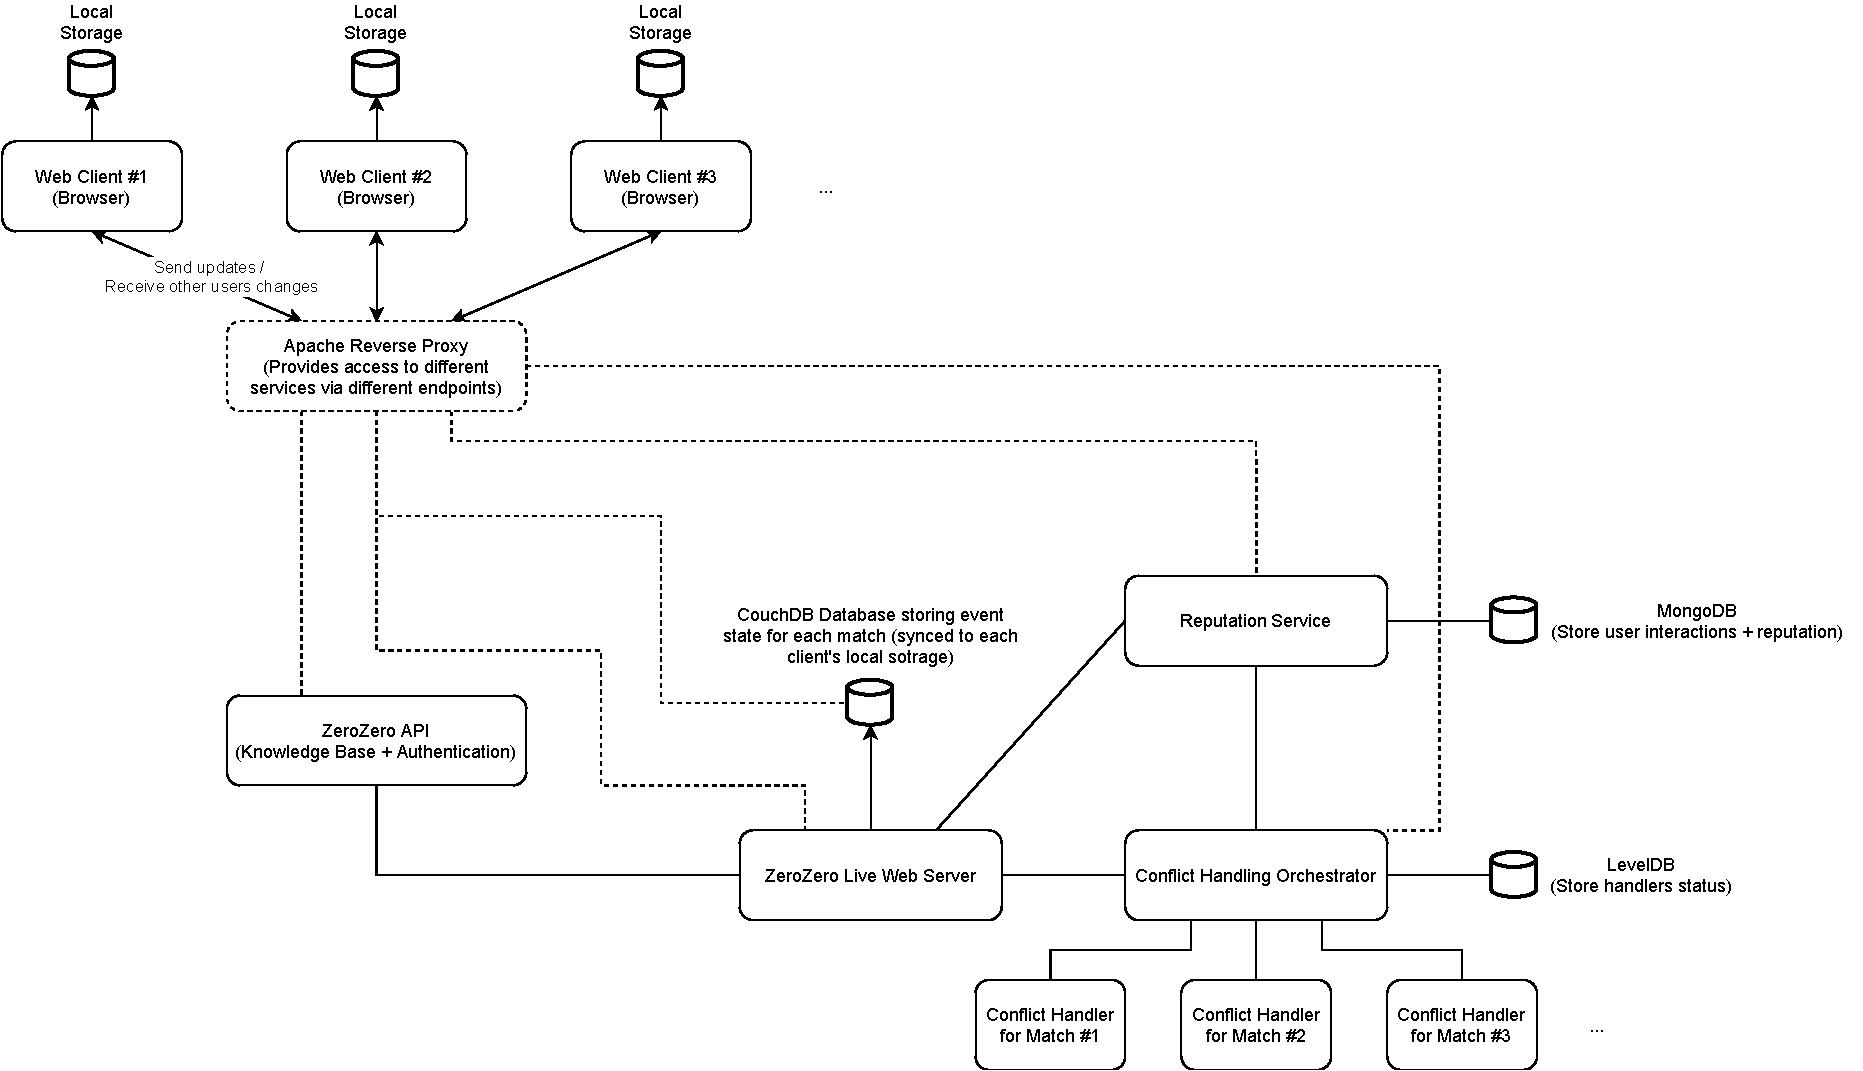
\includegraphics[width=0.5\textheight]{zerozerolive-arch.pdf}
%         % \caption{Services Architecture of the Application}
%     }

%     \end{figure}
    

